\documentclass[main.tex]{subfiles}
\begin{document}

\section*{Method}

To analyze the effects of significant changes to mobility services, we compare the status quo with a hypothetical case that introduces a large fleet of shared demand-responsive vehicles that Cape Town's population may use. Taking advantage of ABM simulations, we are able to deal well with complexity and individual decisions, which gives confidence in the predicted change in congestion we investigate \citep{ronald2015simulating}. 
For this, we fall back to the open source framework MATSim that allows traffic system modeling via ABM. The number of cities with MATsim modeling frameworks and applications has been increasing across the world and includes Bremerhaven, Berlin, S\~{a}o Paulo, Lille Metropolis, Santiago de Chile, Z\"{u}rich, Basel, Vienna, Lagos, Casablanca, Cape Town and the San Francisco bay area \citep{schluter2021impact, maciejewski2016congestion, Kaddoura.2020, sallard2020agent, kickhofer2016creating, balac2021synthetic, diallo2021agent, ilahi2019existing, kagho2019agent, becker2018matsim, muller2021matsim, benhlima2021towards}. 

%Literature on DRT simulation has been investigated by \citealp{ronald2015simulating}, and they highlight ABM to be a valuable tool to simulate DRT before implementing the modeled intervention.

%ABM uses network theory and focuses on individuals in a system, which allows for interaction between operators and users. \\

%because its highly disaggregated level of analysis allows us to investigate the effects of transport policies on travel behavior in a granular way.
 
The upcoming section presents a general overview of MATSim and parameters used in this paper, followed by a description of the Cape Town scenario setup and an overview of the shared mobility scenarios applied.

\subsection*{MATSim framework and scenario parameters}

MATSim represents travellers in the real world as artificial agents with corresponding socio-demographic attributes and aims to mimic real-world travel patterns through an co-evolutionary algorithm \citep{nnene2023simulation}. The framework simulates daily activity and mobility patterns of all agents and takes into account mode choice, departure time and route choice. Movement patterns of road vehicles are simulated on a network graph, which represents local infrastructure and carries attributes such as maximum free speed or road capacity. Interaction between agents on network links with full capacities leads to congestion, which is handled in a queue-based first-in-first-out (FIFO) principle \citep{Horni.2016}. 

An integral part of MATSim ability to reproduce real-world mobility patterns is the optimization of agents' behavior through a maximization of an individual utility score that takes into account the time spent at planned activities and the time and cost spent travelling from one destination to another. In a MATSim simulation, each agent iteratively performs a plan that expresses its preferences in terms of activities, trips and scheduling. Over the course of the iterations, a set of agents modify their plans while others stick to their initial plans. To compare plans with each other, each plan is given a score according to a utility function as described below. The simulation ends after a predefined number of iterations, at which point an equilibrium is reached where no agents can further improve their score.  

The utility function is formulated as follows: 

\begin{equation}
S_{\text{plan}} = \sum_{q=0}^{N-1} S_{\text{activity},q} + \sum_{q=0}^{N-1} S_{\text{travel},\text{mode}(q)}
\label{1}
\end{equation}

with

\begin{equation}
\begin{aligned}
S_{\text{travel},\text{mode}(q)} =\ & C_{\text{mode}} + \beta_{\text{trav},\text{mode}(q)} \times t_{q} \\
& - \beta_{m} \times \left( \gamma_{d,\text{mode}(q)} \times d_{\text{travel},q} + DMC_{\text{mode}} \times \lambda_{\text{mode}} \right) \\
& + \beta_{\text{transfer},\text{mode}(q)} \times x_{\text{transfer},q}
\end{aligned}
\end{equation} 
\\

where $q$ refers to a leg as part of a trip from origin to destination, $C$ is a mode-specific utility constant, and $\beta_{\text{trav},\text{mode}}$ is the marginal utility of traveling per hour (where congestion extends travel time and thus negatively impacts utility). $\beta_{m}$ denotes the marginal utility of money spent on the trip, which equals one throughout the scenario. The term $\gamma_{d,\text{mode}(q)} \times d_{\text{travel},q}$ accounts for distance-based costs (in meters multiplied by a distance rate). Additionally, a daily monetary cost $DMC_{\text{mode}} \times \lambda_{\text{mode}}$ is incurred. Here, $\lambda_{\text{mode}}$ is a boolean variable that equals 1 if the agent uses a particular mode for the first time on a given day and 0 otherwise. This fee can be interpreted as representing vehicle fixed costs or subscription fees for public transport or demand-responsive transport (DRT).  $\beta_{\text{transfer},\text{mode}} \times x_{\text{transfer},q}$ represents a transfer penalty applied when agents must switch vehicles within a trip leg (e.g., for public transport legs) \citep{Horni.2016}. 

Table~\ref{Utility values} lists the mode-specific utility values and pricing parameters used for Cape Town. Mode-dependent utilities for agents in Cape Town were established by adjusting values of the well-established Berlin scenario \citep{Ziemke.2019} until mode share and congestion calibration targets of Cape Town were met to match local sociodemopgrahic characteristics and travel dynamics (for further information on the calibration excercise, see section below).

\begin{table}[H]
\centering
\resizebox{1\textwidth}{!}{%
\large % Hier wird die Schriftgröße geändert
\begin{tabular}{|l|p{2cm}|p{3cm}|p{4cm}|p{3cm}|p{3cm}|}
\hline
\textbf{Mode}             & \textbf{Constant ($C$)} & \textbf{Daily monetary constant (DMC)} & \textbf{Marginal utility of travelling ($\beta_{\text{trav}}$) } & \textbf{Monetary distance rate (ct/km) ($\gamma_{d})$} & \textbf{Transfer utility ($\beta_{transfer}$)} \\ \hline
Public transport & 0 & -1.9 & 0 & 0 & -1 \\ \hline
Car              & 0 & -10 & 0 & -11 & 0 \\ \hline
DRT              & 0 & varying & 0 & varying & 0 \\ \hline
\end{tabular}
}
\caption{Varying utility and pricing parameters for different transportation modes available in the simulation}
\label{Utility values}
\end{table}

It becomes evident that, under this modeling setup, travel time using a particular mode does not directly impact an agent's (dis)utility while traveling. However, longer travel times reduce the time available for activities (captured by the first term in equation~\ref{1}), indirectly lowering the agent’s overall score. Consequently, agents will seek to avoid traffic congestion, as increased travel time decreases their utility. We explicitly acknowledge, however, that Cape Town travellers may exhibit additional behavioural inertia (e.g., distrust in shared or public rides or preference for private-car autonomy even under congestion) that is not fully captured by the utility function. The simulation outcomes should therefore be interpreted as the potential congestion relief if mode choice behaviour aligns with the modelled rational response. \textcolor{red}{Reviewer critic Cannibalization modelling: Make it clear that agents can or cannot perform intermodal mobility trips (i.e. different mode legs during a trip) }

\subsection*{\textcolor{red}{Explain MATSIM-internal DRT mechanism}}

\subsection*{Baseline Cape Town MATSim-scenario and Calibration}

A synthetic scenario of Cape Town with a population sample size of 10\,\% is employed for the study. We derive the synthetic population from South African Census Data 2011 \citep{census2011}, the 10\,\% Public Use Sample \citep{census2011public10pct} and the Minnesota Population Center Integrated Public Use Microdata Series \citep{mpc2020}. For the population synthesis process we employ a multi-level iterative proportional fitting methodology.  Furthermore, we utilize data from National Household Travel Survey 2013 \citep{nhts2013} and the Time Use Survey 2010 \citep{tus20NationalHouseholdTravelSurvey13} to assign individual mobility behaviour to the synthetic agents. 

On the supply side we employ network and infrastructure data from OpenStreetMap (OSM) \citep{osm}. The network links are downscaled according to the population sample in terms of flow and storage capacities. Furthermore, the individual OSM IDs of the dataset are extracted and categorised into different activities such as "shopping" or "leisure". In addition, we use GTFS datasets from the main public transport providers in Cape Town from 2018 to model public transport \citep{transifeeds}. The capacities of the public transportation vehicles are also downscaled according to the population sample (1:10), as the adjustment of the vehicle size to the downscaled network leads to a distortion of the passenger flows. To avoid further distortions in the timetables of the vehicles by the other network participants and for reasons of simplification, the vehicles of Golden Arrow Bus Services (GABS), Metrorail Western Cape, MyCiTi Cape Town Integrated Rapid Transit (IRT) system and the University of Cape Town's (UCT) campus shuttle buses operate on a pseudo-network with direct aerial lines between stops and with adjusted speed limits on each route to match the timetable. For the modelling of informal public transport in the form of minibus taxis, the use of a pseudo-network is omitted due to the fact that the number of minibus taxis is significantly higher than in the case of formal public transport which leads to feedback effects in the traffic flow. To represent these effects in the overall traffic in Cape Town the Minibus Taxis travel together with the other individual traffic on the OSM motor roads. 

Again, using the OSM data, the modelled infrastructure and the socio-demographic characteristics of the agents such as age, gender and employment status, a gravity model is used to create a path-destination matrix and assign it to the agents. The resulting base population then goes through several calibration steps to accurately mimic the real world travel patterns, calibrating towards NHTS averages and Cape Town Vehicle Detection System (VDS) traffic flow data on major roads from 2018. The calibration target is set at an average deviation from real data of less than 20\,\% error for car traffic and less than 50\,\% for formal and informal public transport.

Figure \ref{fig:x_1} shows the location of traffic count station the simulation was calibrated against. Moreover, it depicts the average free flow speed divergences in km/h on major streets during a weekday rush hour between 4 and 5 pm based on TomTom traffic analysis data from October 2022. Figure \ref{fig:x_2} shows calibration results of an example count station. This goes to show that the model is fit well against major mobility patterns, in particular traffic delays.

\begin{figure}[H]
\centering
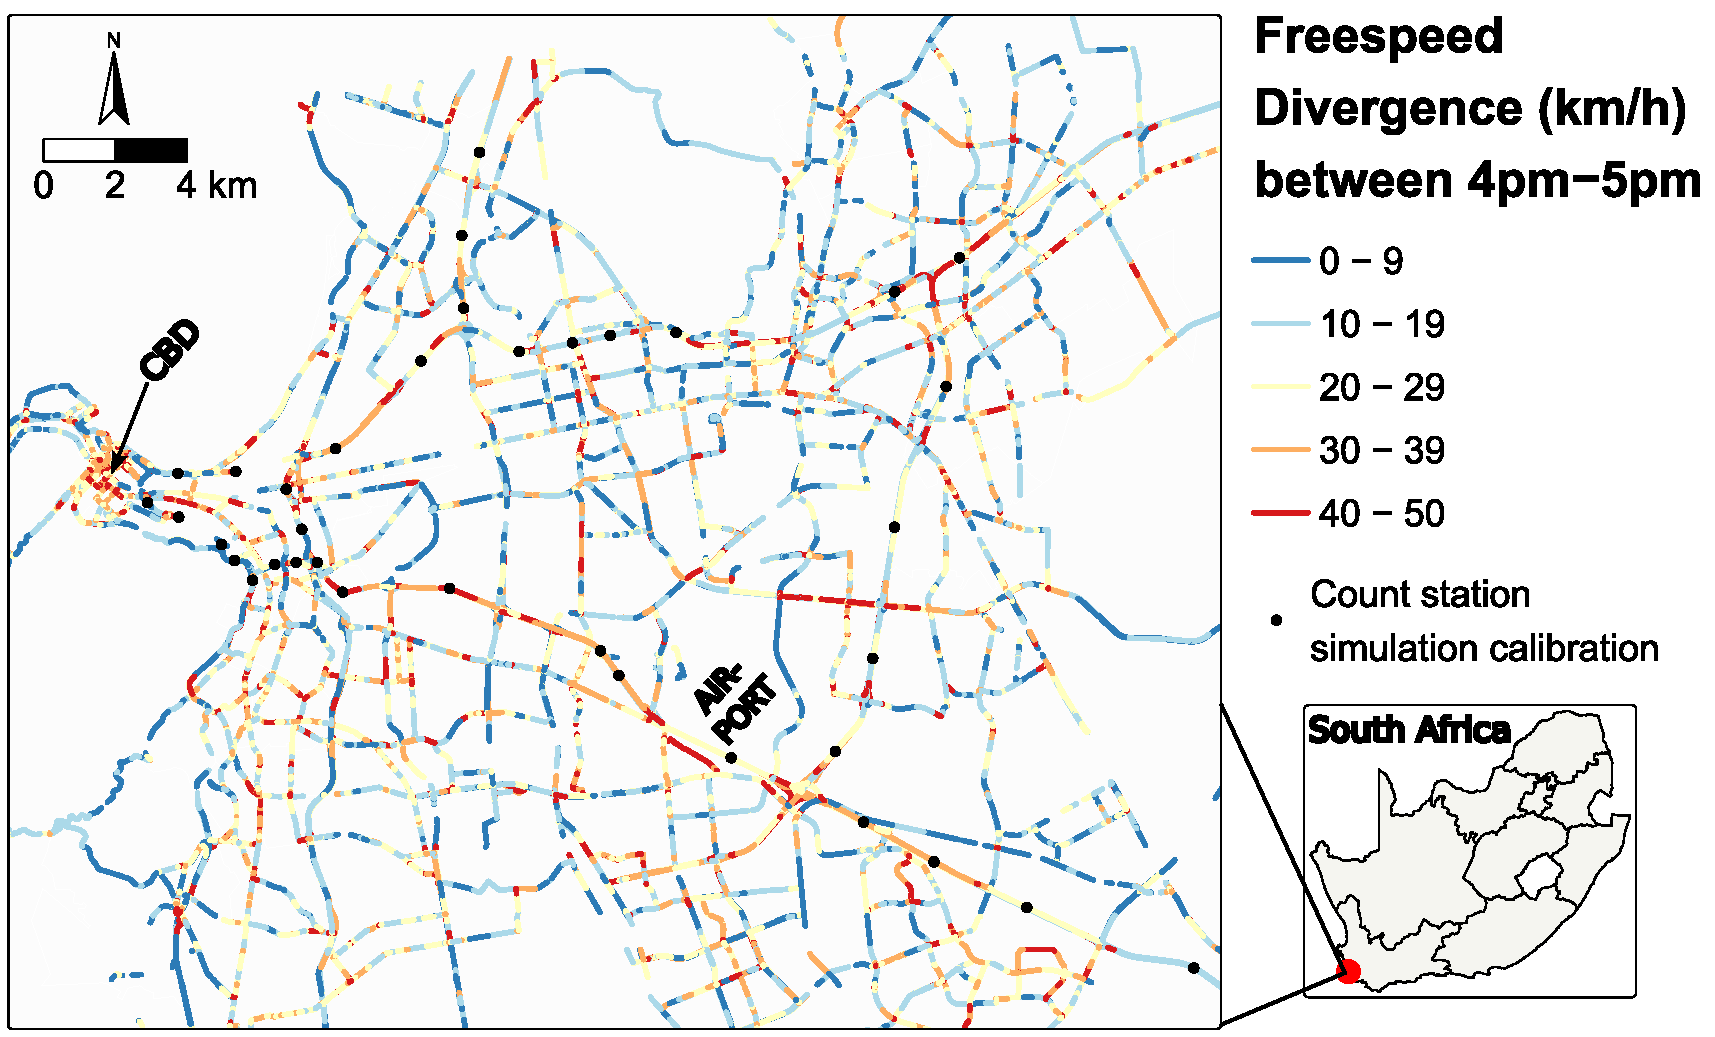
\includegraphics[width=1\textwidth]{images/Meine_Karte_mit_Inset_22_cropped.pdf}
  \captionsetup{width=.8\textwidth}
  \caption{Free flow speed Divergence on Major Roads in Capetown on an Average Wednesday in October 2022 for Capetown (Data: TomTom). Points depict traffic count stations that have been used to calibrate the simulation}
  \label{fig:x_1}
\end{figure}

For our chosen measure of traffic congestion, the difference between the free flow speed and the actual simulation flow speed is aggregated for each street link on a daily basis. As noted earlier, since scheduled transport operates on artificial links that have no intersections with links corresponding to the real world, we account only for congestion caused by cars and minibus taxis, which make up the vast majority of traffic on Cape Town's streets.

\begin{figure}[H]
\centering
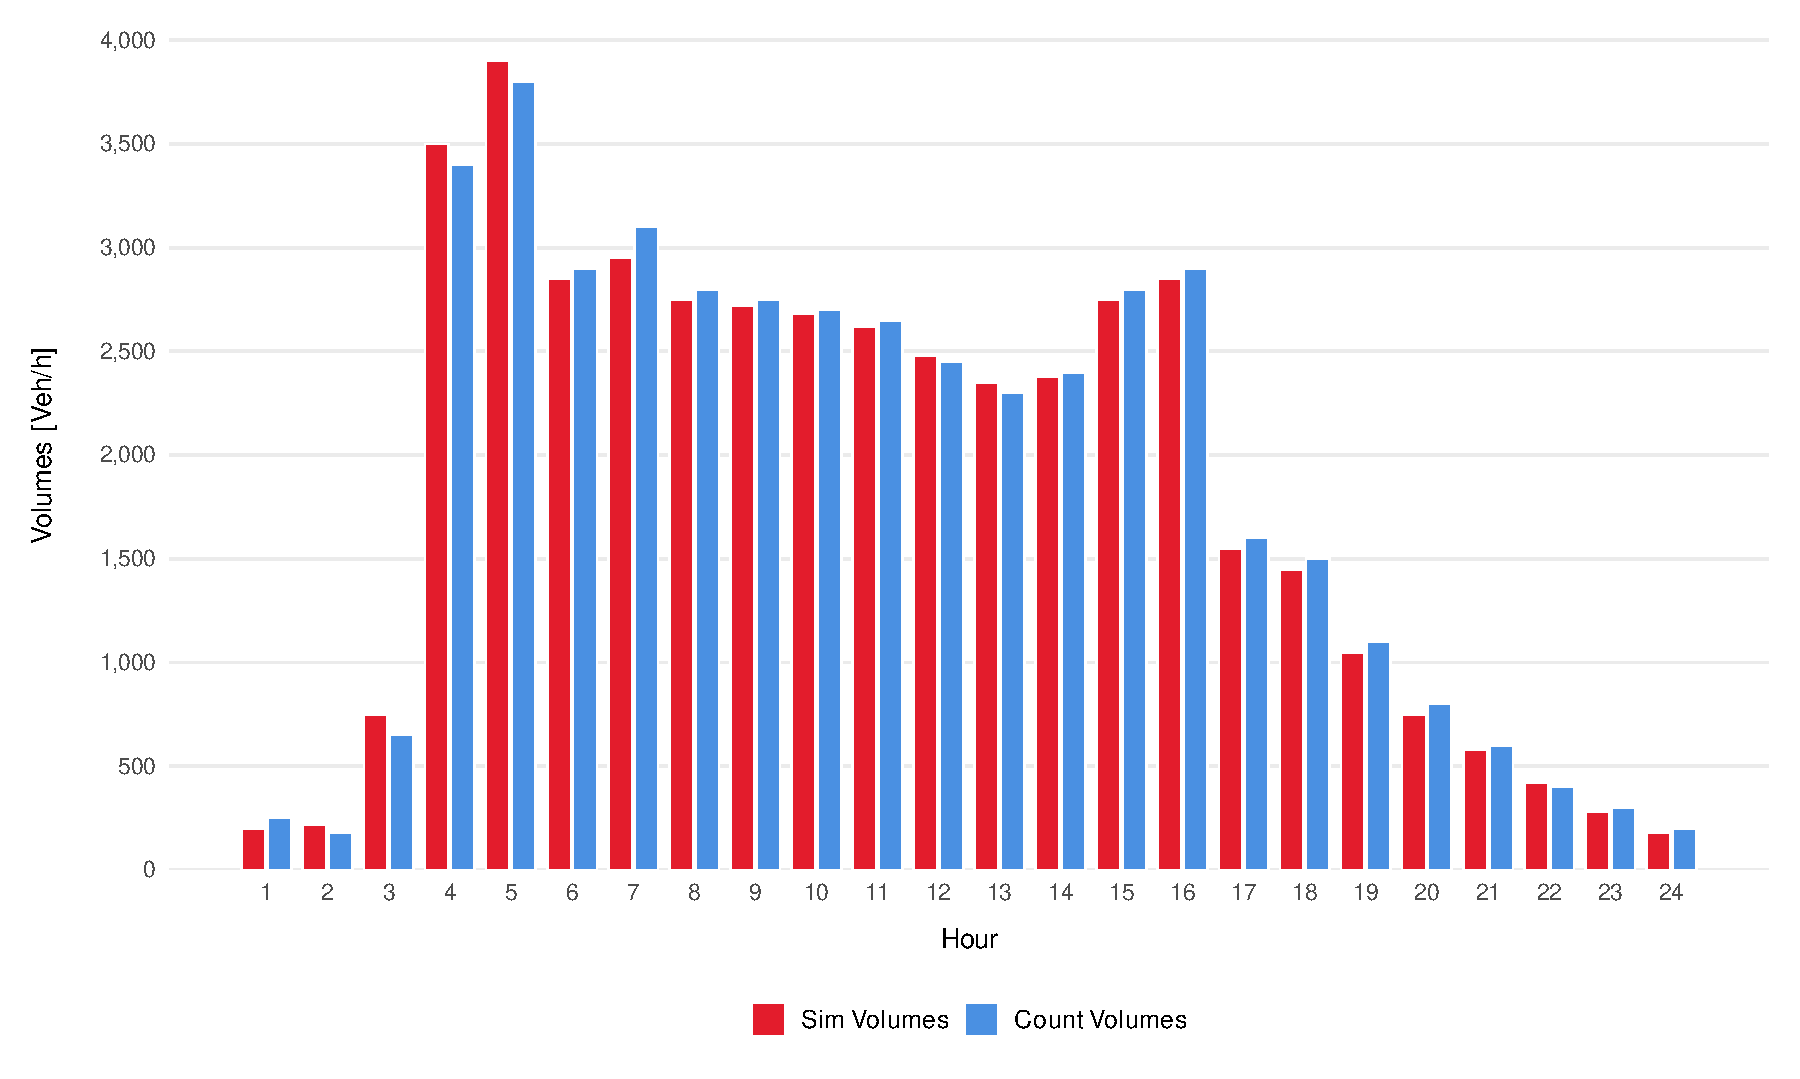
\includegraphics[width=1\textwidth]{images/airport_count_station.pdf}
  \captionsetup{width=.8\textwidth}
  \caption{Simulation Calibration Results for Traffic Count Station near Airport}
  \label{fig:x_2}
\end{figure}



\subsection*{DRT scenarios \& parameterization} 

The main objective of this study is to analyze whether introduction of a large-scale DRT fleet is able to reduce congestion by encouraging a modal shift from private cars to DRT while prevent public transport cannibalization by the new introduced mode. To achieve this, we design a service area where agents who begin or end their trips within the designated area have the option to switch to DRT. Other service type options like the introduction of a stop-based DRT system are not considered because they would resemble the existing paratransit systems to a large extent. In our service-area based approach, agents can ride-hail DRT vehicles when the start and end of their trip falls within the defined service area.   

We design the DRT service area using a two-step process. First, we identify wards with the highest car trip activity. Second, we combine these with wards that have a high concentration of upper-middle-income households to create a final service area that captures a large share of car trips while targeting users who are more likely to afford and use the service.

Using origin-destination car trip data from TomTom (2022), we calculate the share of inter-ward car trips for every origin-destination ward pair in Cape Town. We rank these ward pairs in descending order based on their contribution to total car trips and compute the cumulative share. By applying a 60\,\% coverage threshold, we select all wards that appear in at least one of the top-ranked origin-destination pairs. Figure~\ref{fig:x_5} shows the spatial distribution of car trip origins. Car usage remains particularly high in the more affluent suburbs surrounding the city's major economic hubs (CBD, Kenilworth, and Bellville).

\begin{figure}[!h]
\centering
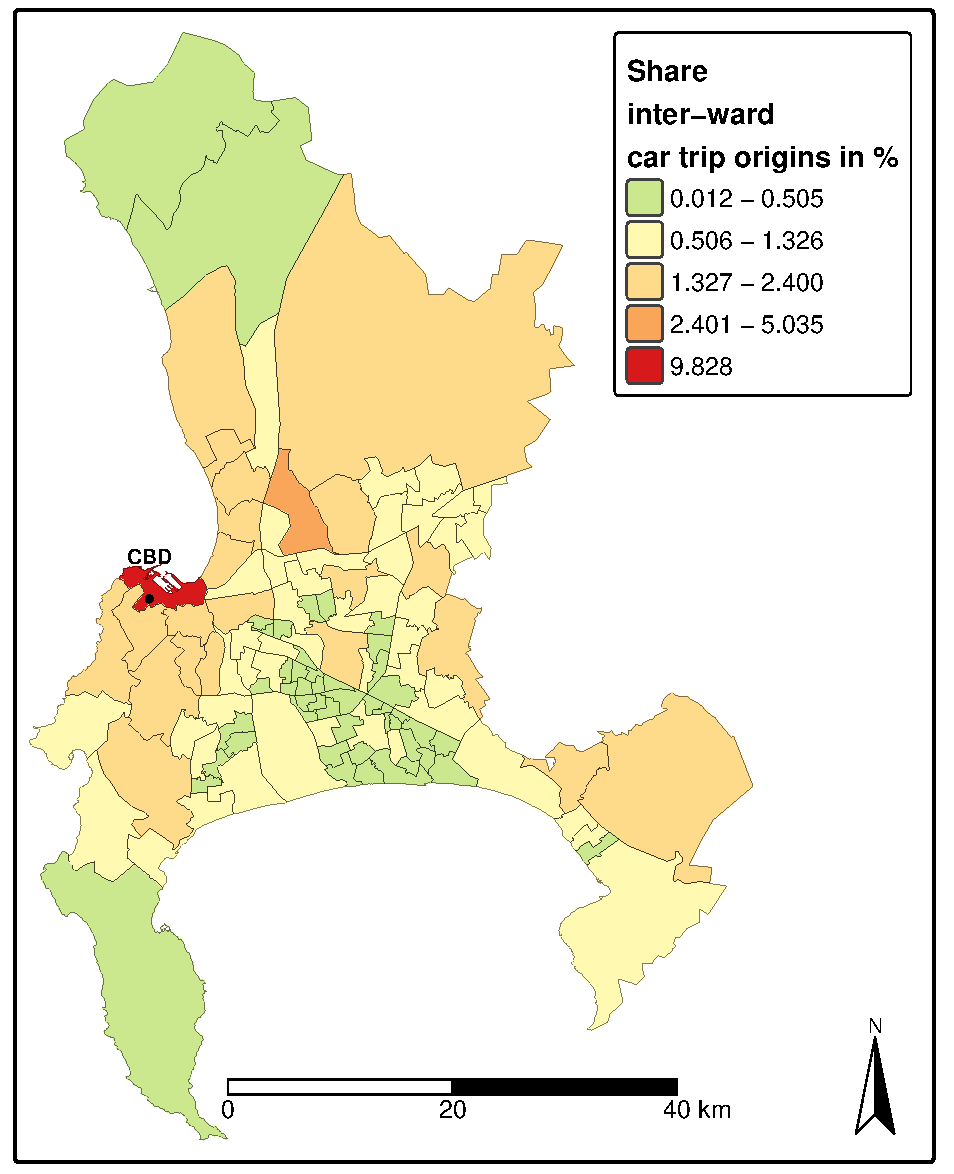
\includegraphics[width=0.6\textwidth]{images/inter-wards_car_trips_origins_edit-3_cropped.pdf}
\captionsetup{width=.9\textwidth}
\caption{Share of inter-ward car trip origins per ward in \% (Data: TomTom 2022)}
\label{fig:x_5}
\end{figure}

DRT functions as a hybrid between public transportation and private car use. Therefore, its fares are expected to be higher than conventional public transport but lower than the full cost of driving a private car. We target neighborhoods with a high concentration of upper-middle-income households that have greater financial capacity to pay for a higher-quality on-demand service. Additionally, market-based solutions like DRT could help alleviate the lack of public infrastructure \citep{TDCIP}. Using data from the 2011 South African Census \cite{census2011}, we identify wards with the highest share of upper-middle-income households (annual household income between ZAR\,76 801 and ZAR\,614,400, \$13,798.24 – \$110,384.5 PPP). These wards are then combined with the high car-usage wards from Step 1 to define the final DRT service area.

This service area, marked by the blue boundary in Figure~\ref{fig:x_3}, covers 83.7\,\% of all origin-destination car trips recorded by TomTom, making it a well-targeted region with high car traffic, congestion, and private car usage, particularly in key business centers across the city. The same figure also shows the baseline (no-DRT) traffic congestion levels in the study area. In the baseline scenario, congestion causes approximately 253,000 hours of additional travel time, accounting for 86\,\% of total car travel time in the region. Congestion inside the designated DRT service area (131,500 hours) is slightly higher than outside it (121,500 hours).

%\begin{figure}[!h] \centering 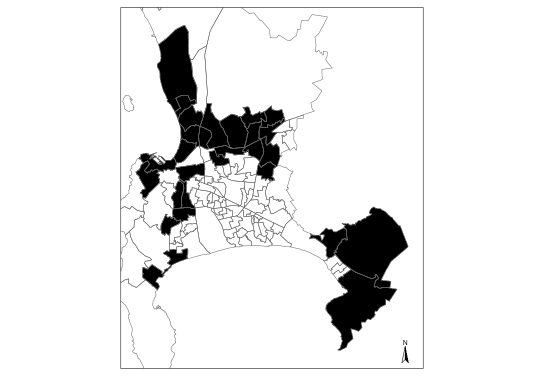
\includegraphics[width=1\textwidth]{images/service_area.png} \captionsetup{width=.9\textwidth} \caption{DRT Service Area} \label{fig:x_6} \end{figure}

\begin{figure}[H] \centering 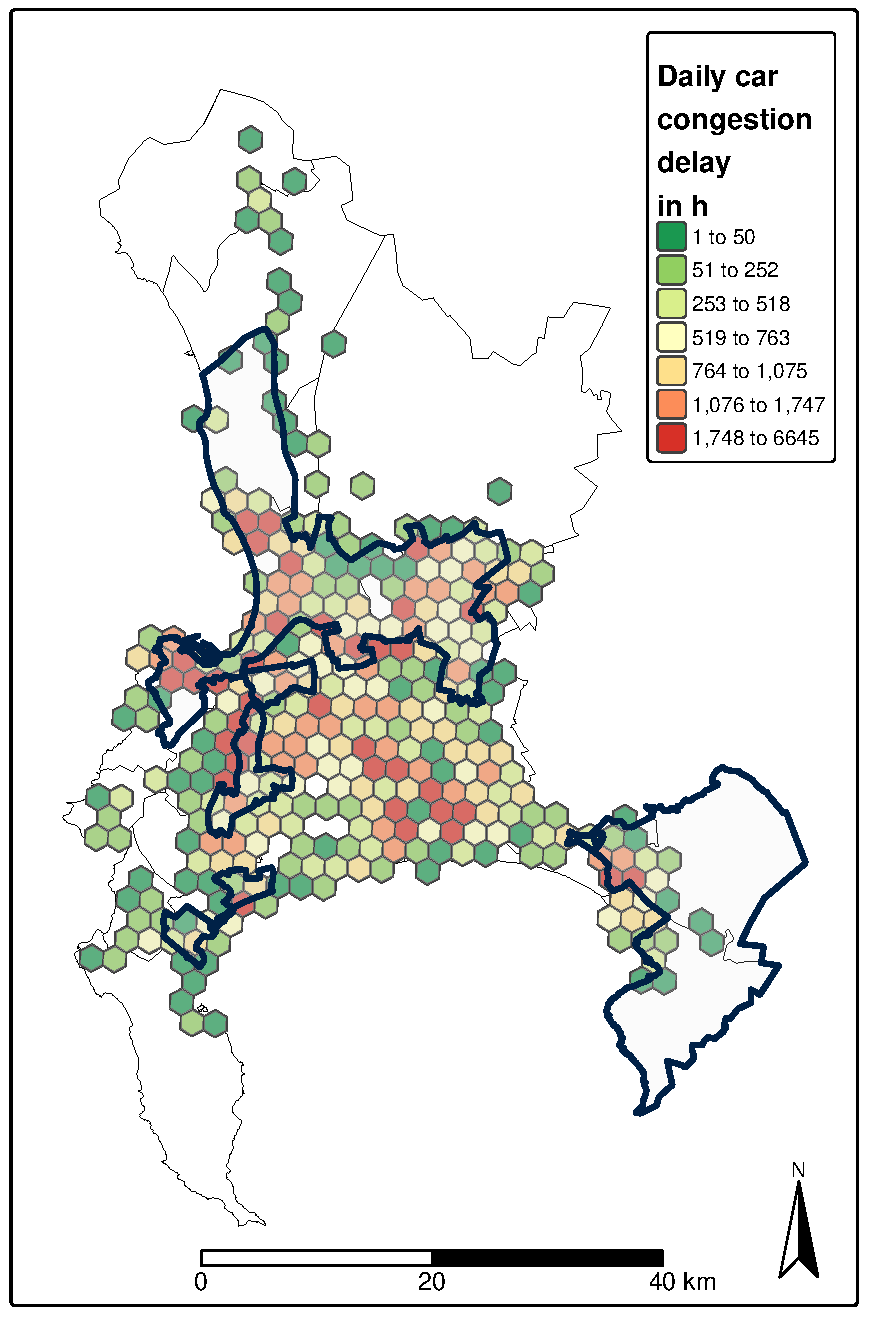
\includegraphics[width=0.6\textwidth]{images/daily_delay_basecase_edit-3_cropped.pdf} \captionsetup{width=.9\textwidth} \caption{Simulation baseline scenario: Spatial distribution of daily congestion. The blue-highlighted area marks the DRT service area constructed} \label{fig:x_3} \end{figure}

%\begin{figure}[H] \centering 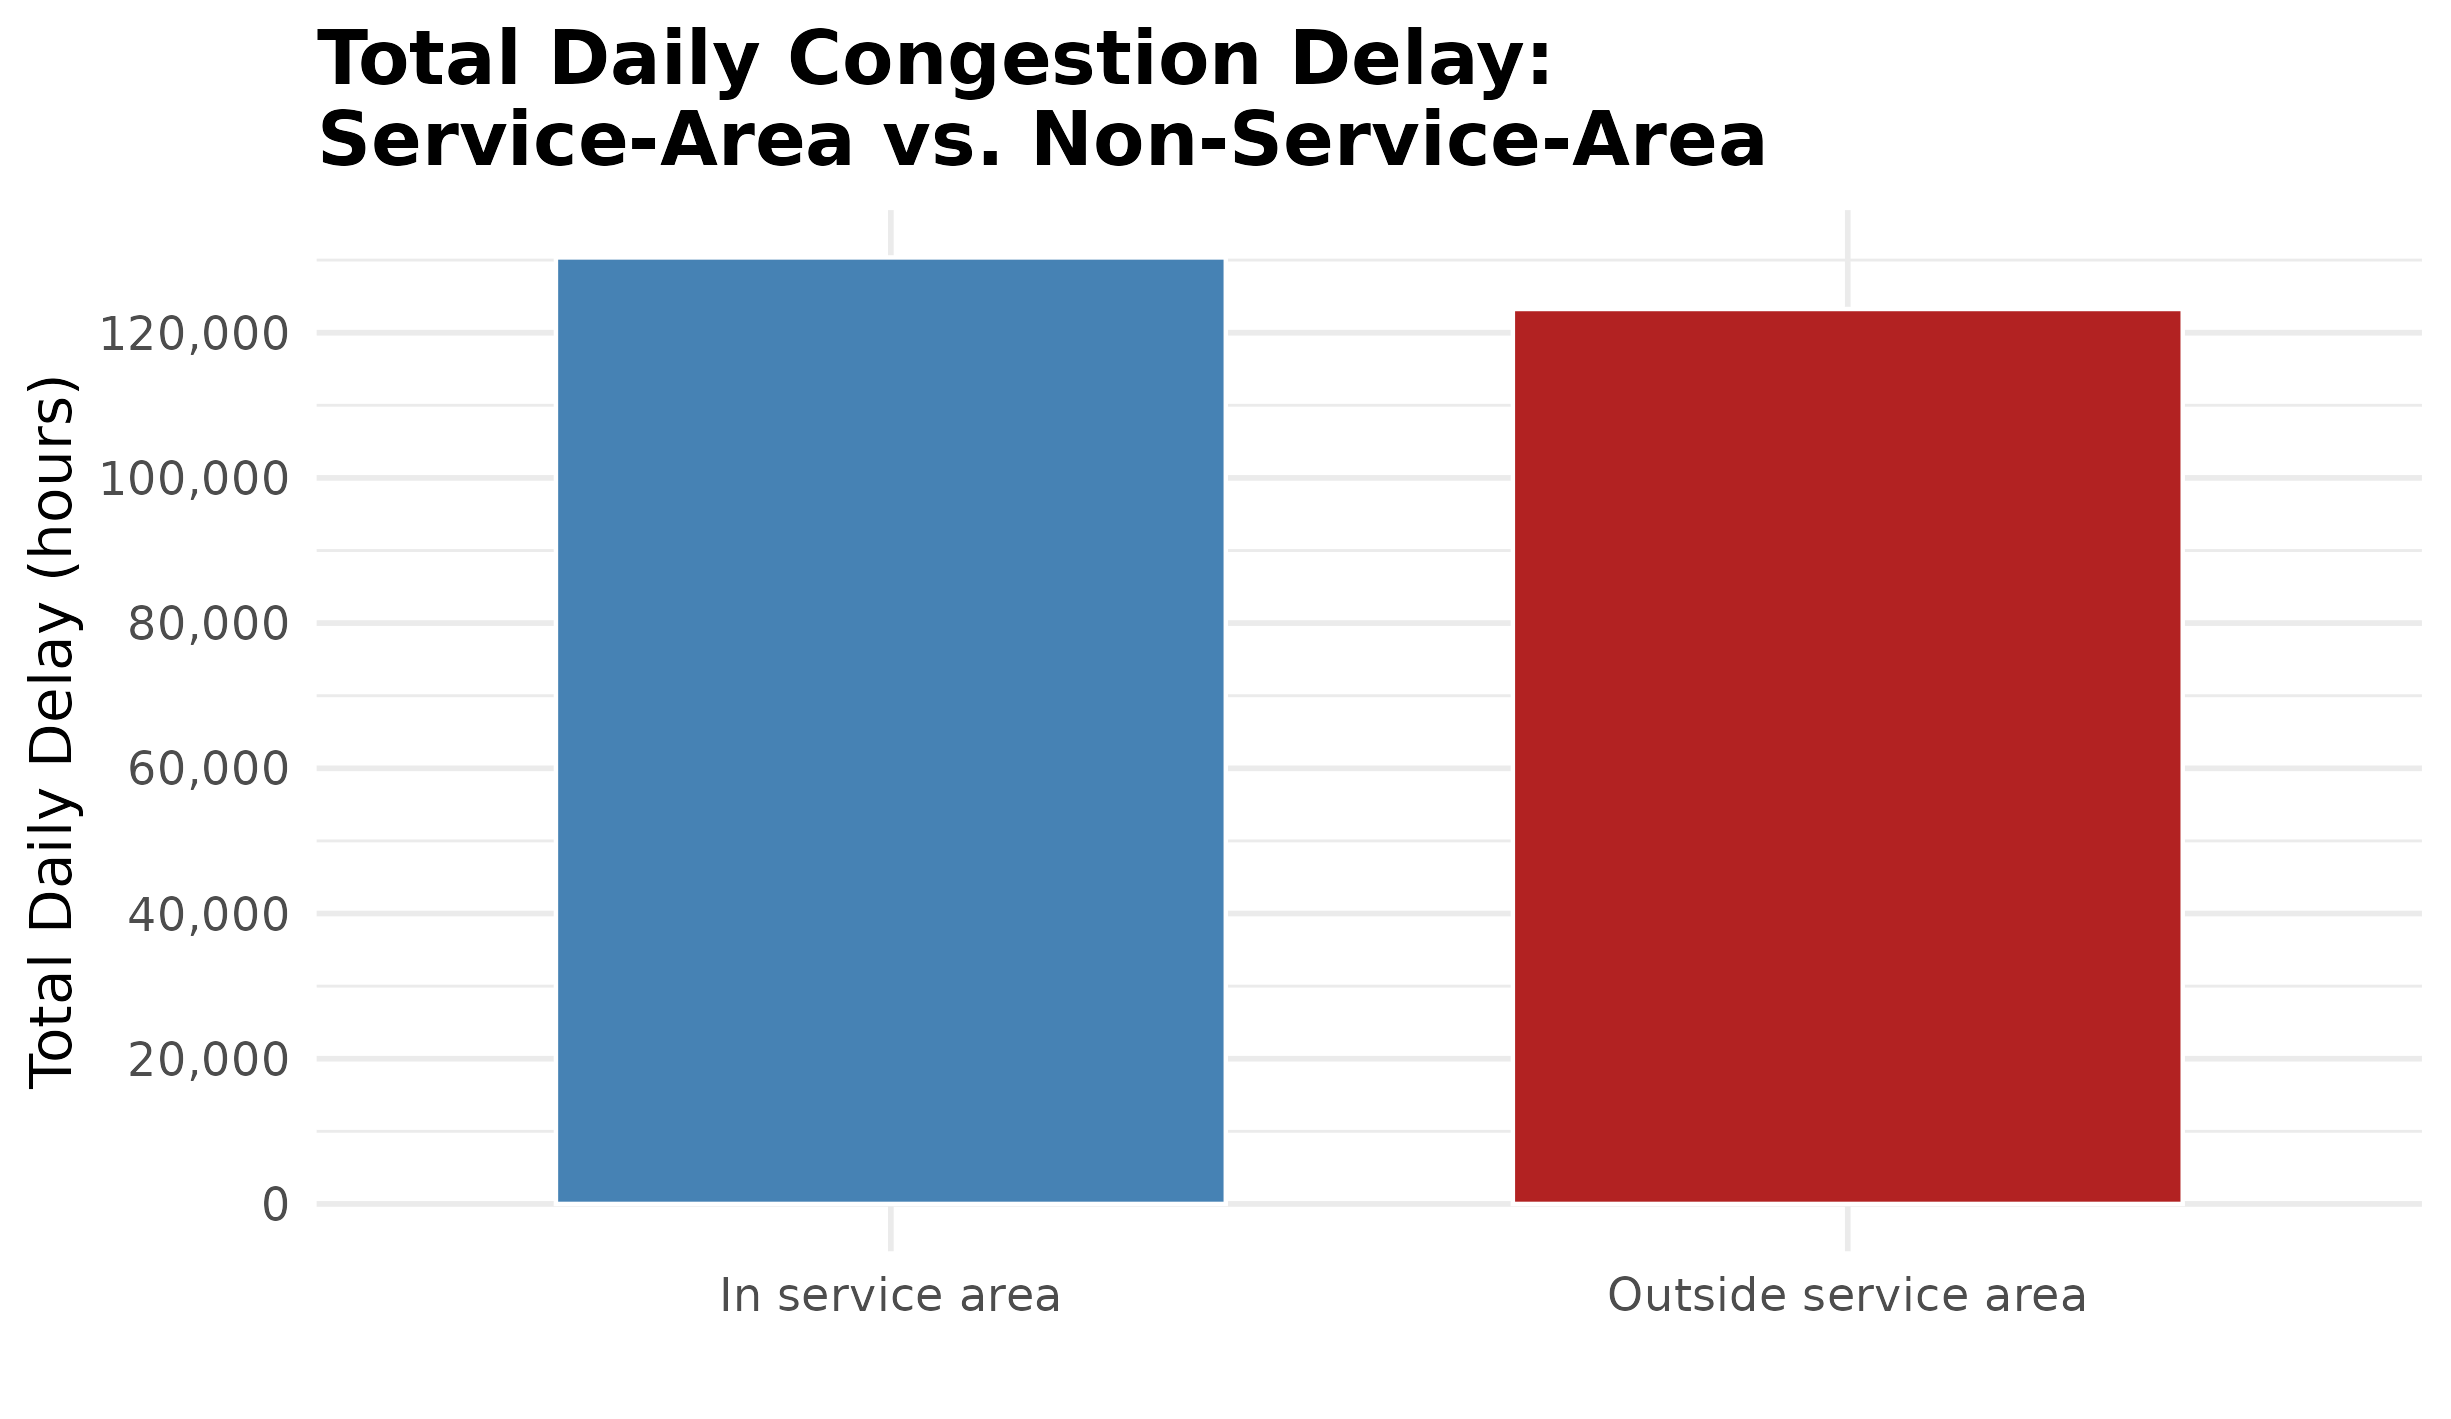
\includegraphics[width=0.8\textwidth]{images/baseline_total_congestion_service_area.png} \captionsetup{width=.9\textwidth} \caption{Simulation baseline scenario: Aggregate daily congestion in and outside of DRT service area} \label{fig:x_4}  \end{figure}

Several scenarios using different fleet sizes and pricing schemes are simulated to evaluate the potential impact on congestion. The fleet sizes are based on a sample of total car drivers in the baseline MATSim scenario (52,775 drivers, or a 10\,\% sample). We test fleet sizes equivalent to 0.5\,\%, 1\,\%, 1.5\,\%, and 2\,\% of the total car drivers in Cape Town (264, 528, 792, and 1056 vehicles, respectively).

The pricing factor plays an essential role in shaping the choice of service areas. Since higher-income areas are more likely to afford transport options that are priced higher than public transport, while lower-income areas already spend significant portions of their income on public transport, the pricing is adjusted to reflect these differences. 
For the DRT pricing schemes, we vary both the mandatory one-time daily fee and the variable price per kilometer. The daily fee is set to 200\,\%, 250\,\%, and 300\,\% of the daily fixed fee for public transport, while the variable distance price takes up the values from 45.45\,\%, 55.55\,\%, 65.65\,\%, 75\,\% and 100\,\% of the car km fee used in the baseline scenario. Notably, the pricing structure of the DRT services deviates from ride-hailing services like Uber or Bolt in that the variable cost for shared DRT rides are split between the two or more passengers, making the trip cheaper than ride-hailing services on the same route. Table \ref{tab:drt_parameters} presents all parameter dimensions and relevant values. In total, we evaluate 60 different scenarios based on all value combinations of the parameter dimensions.\\

\begin{table}[h]
\centering
\resizebox{1\textwidth}{!}{%
\begin{tabular}{c|c|c}
\hline
\textbf{Fleet size (\% of daily car drivers)} & \textbf{Daily DRT fee (\% of PT daily fee)} & \textbf{Variable DRT fee (\% of car km fee)} \\
\hline
0.5\,\%, 1.0\,\%, 1.5\,\%, 2.0\,\% & 200\,\%, 250\,\%, 300\,\% & 45.45\,\%, 55.55\,\%, 65.65\,\%, 75\,\%, 100\,\% \\
\hline
\end{tabular}
}
\caption{Complete parameter grid for all 60 simulated DRT scenarios}
\label{tab:drt_parameters}
\end{table}

The pricing assumptions were selected to reflect realistic affordability thresholds for upper-middle-income households in Cape Town, who are more likely to adopt DRT as a viable alternative to private cars or existing ride-hailing services. The daily fee levels were chosen as they represent a midpoint between low-cost public transport and higher car ownership costs (the latter being more than five times as high than the former), allowing us to observe the intended mode-shifting effects without making DRT prohibitively expensive. For instance, a 200\,\% daily fee aligns with real-world pricing in similar contexts, such as Hamburg's MOIA service, where fares are approximately 2–3 times public transport rates to encourage uptake among affluent users \citep{KagerbauerKostorzWilkes2021_1000141282}. The variable distance rates (45.45\,\% to 100\,\% of car km fees) enable further sensitivity analysis, specifically designed to test DRT's competitiveness below the full variable costs of cars. By setting rates as low as 45.45\,\% (e.g., equivalent to a subsidized or efficiency-optimized fare), we capture scenarios where DRT incentivizes shifts from private cars—whose variable costs include fuel and maintenance—while remaining attractive relative to ride-hailing services like Uber or Bolt, which often charge 80–120\,\% of car km equivalents due to unshared rides and surge pricing \citep{Tirachini2020-sr}). Higher rates (up to 100\,\% of the variable car price) simulate less subsidized operations, revealing potential thresholds where adoption drops and congestion relief diminishes. 



\end{document}